\documentclass{tikzposter}
\usepackage{jgu_tikzposter}

\title{Retention Time Alignment}
\institute{University Medical Center, Johannes Gutenberg University, Germany}
\author{Mateusz Krzysztof Łącki, Ute Distler, Stefan Tenzer}
\insertlogo[width=10cm]{img/jgu3.pdf}
\insertqr[3in]{https://github.com/MatteoLacki/rta}

\begin{document}
\maketitle

\begin{columns}
\column{0.5}


\block{Rationale}{
	\begin{itemize}
		\good LC-IM-MS instruments identify thousands of peptides obtained from digested proteins
		\bad most observed signals are not easily sequenced and are useless in the identification process
		\good one can retrieve a lot of unidentified signals by x-annotation!
	\end{itemize}
	\begin{tikzfigure}
		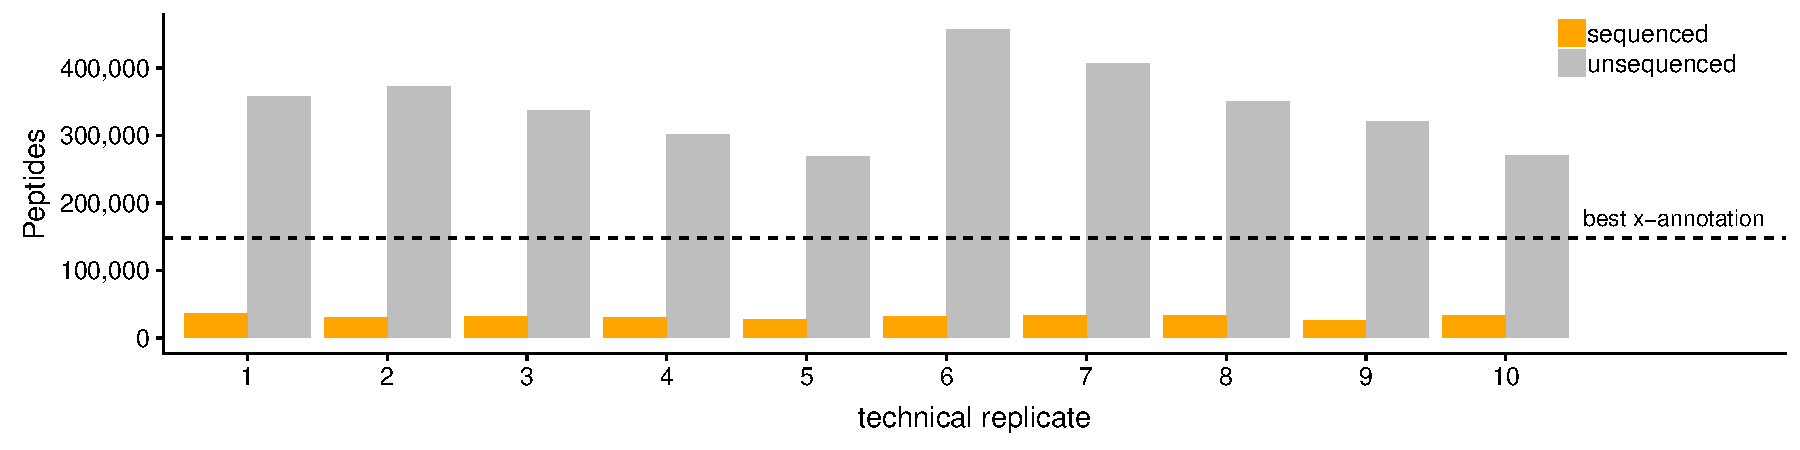
\includegraphics[width=\linewidth]{R/img/x-annotation.pdf}
	\end{tikzfigure}

	\begin{itemize}
		\ugly technical replicates reveal not always the same peptides
		\good biochemical properties of signals in different runs are similar
	\end{itemize}
	
	\begin{tikzfigure}
		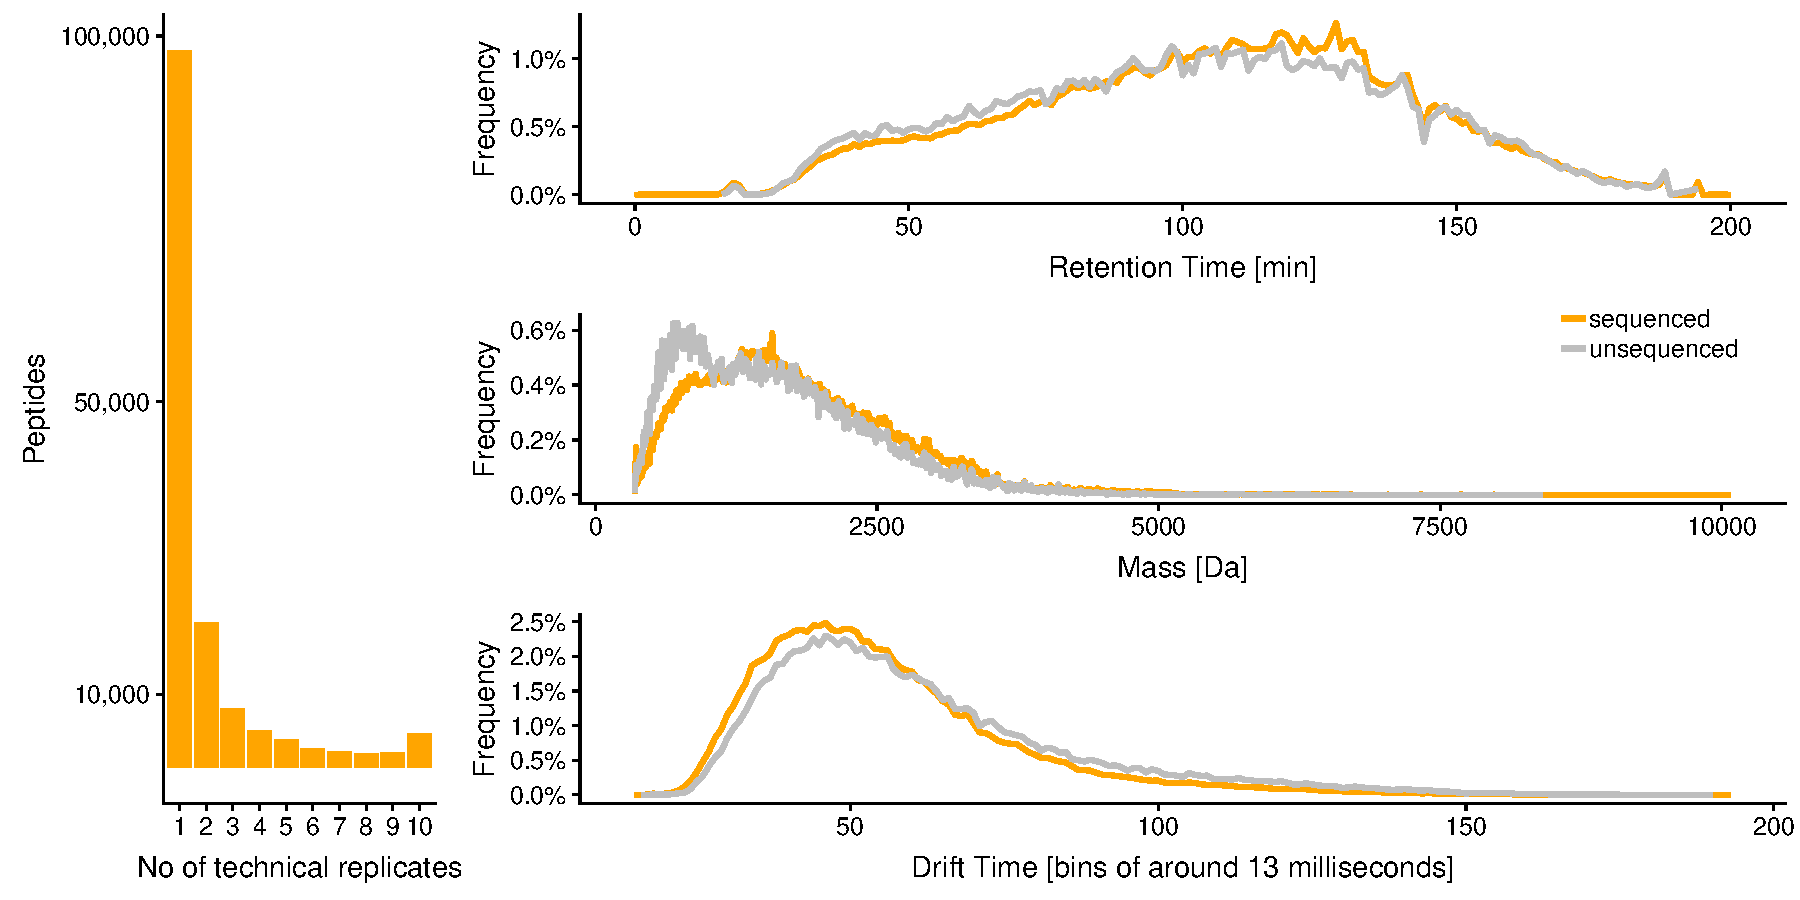
\includegraphics[width=\linewidth]{R/img/venn_and_similarfeatures.pdf}
	\end{tikzfigure}

	\begin{itemize}
		\bad retention times accross technical replicates do show significant systematic deviations
		\bad some sequenced peptides differ significantly between runs (mostly by few minutes)
	\end{itemize}

	\begin{tikzfigure}
		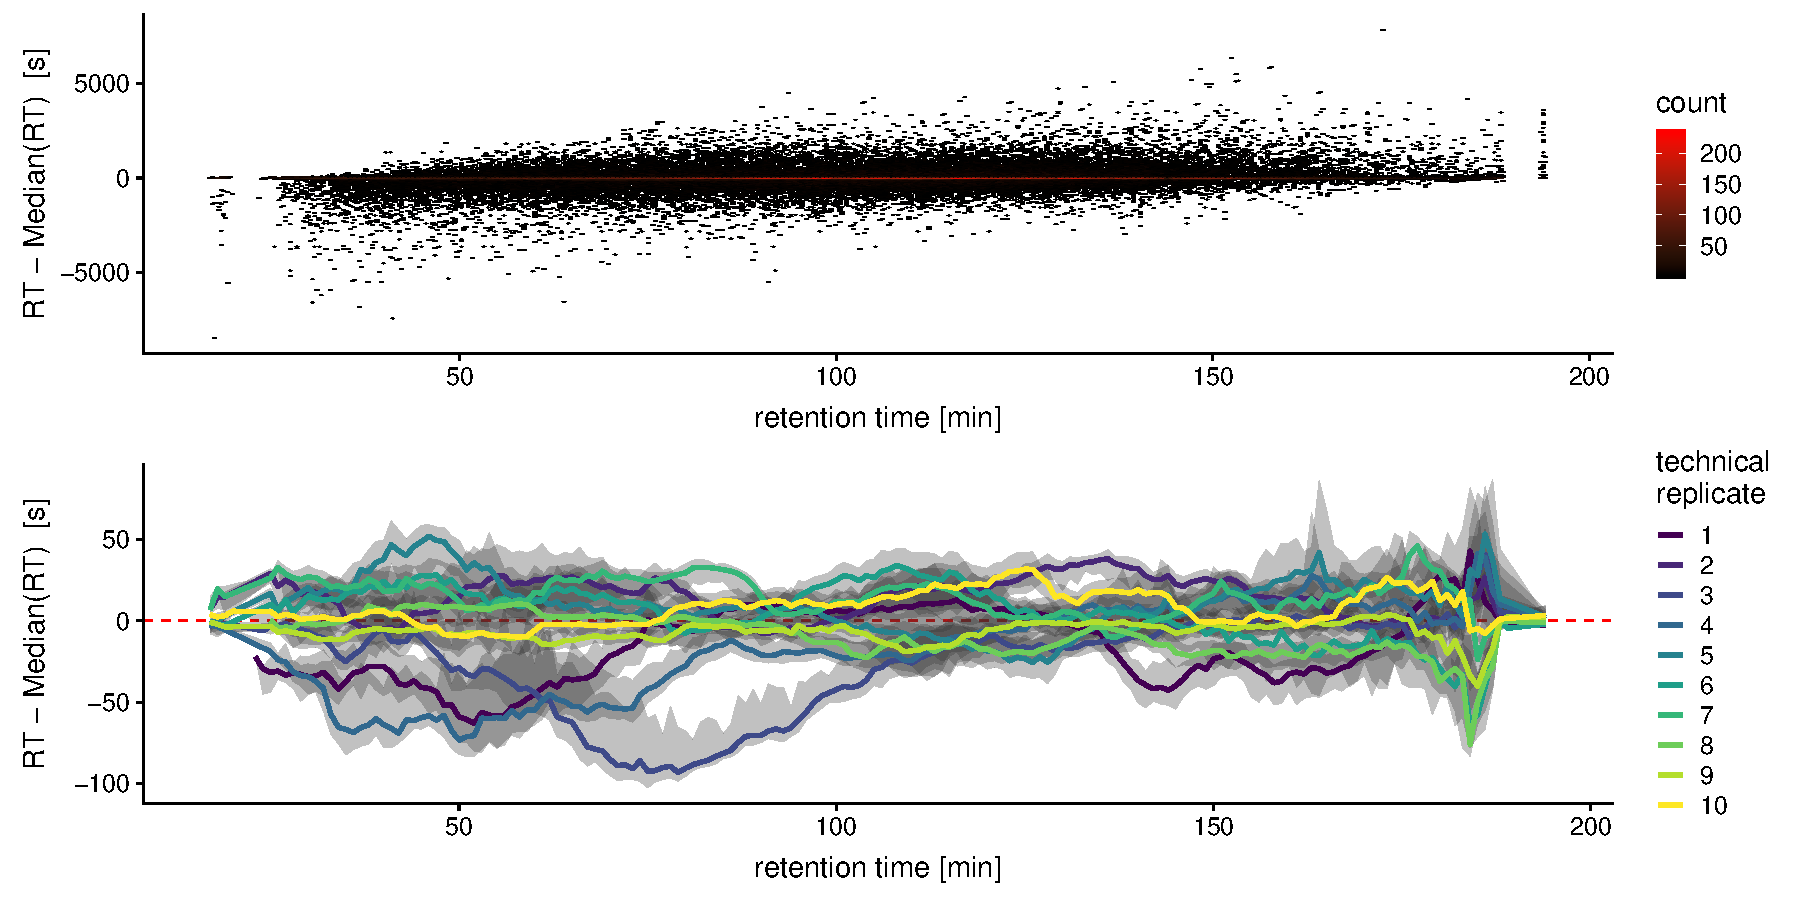
\includegraphics[width=\linewidth]{R/img/rt_dists.pdf}
	\end{tikzfigure}
} 

\block{Retention Time Alignment to the rescue!}{
	\begin{itemize}
		\item our task is to adjust the retention times observed across $S$ technical replicates
		\item we construct $S$ \texttt{alignments}, i.e. functions $F_s: \mathbb{R}_+ \rightarrow \mathbb{R}_+$ that act on the retention times of observed peptides measured at different technical replicates, $RT_{sp}$, where
		\begin{itemize}
			\item $s = 1,\dots,S$ is a technical replicate number
			\item $p$ denotes a peptide from all observed peptides $\mathfrak{P}$
		\end{itemize}
		\item the \texttt{alignments} $F_s$ must meet some requirements. In particular, they must be
		\begin{itemize}
			\item strictly increasing, as otherwise they could glue some some $RT_{sp}$
			\item not influenced much by the miss-assigned peptides
		\end{itemize}
	\end{itemize}
	% \begin{itemize}
	% 	\good our tasks are:
	% 	\begin{itemize}
	% 		\item filter out the miss-assigned peptides
	% 		\item get rid of the systematic deviations
	% 	\end{itemize}
	% 	\good 
	% \end{itemize}

	% \coloredbox{
	% 	hhah
	% }
}



\column{0.5}


\block{Other similar approaches}{
	\begin{itemize}
		\bad the idea of the retention times alignment is not new
		\begin{itemize}
			\item the \texttt{Match Between Runs} has been a standard part of \texttt{MaxQuant}\cite{tyanova2016maxquant}
			\item presented solutions simplify some of the procedures already present in \texttt{IsoQuant}\cite{distler2013drift,kuharev2015depth}
		\end{itemize}
		\ugly retention time alignment used in \texttt{IsoQuant} is not based on the MS-based identifications
	\end{itemize}
	
	

}

\block{Literature}{
	\bibliographystyle{plain}
	\bibliography{bib/spectrometry}
}
\end{columns}

%\note{Notetext} % See Section 4.3
\end{document}
